\documentclass{source/Report}
\usepackage{caption}
\usepackage{multirow}

\major{信息工程}
\name{张卓雨}
\title{}
\stuid{3210105816}
\college{信息与电子工程学院}
\date{2023年3月28日}
\lab{东四-224}
\course{电磁场与电磁波}
\instructor{吴锡东、王子立}
\grades{}
\expname{微带传输线负载特性矢网测量}
\exptype{}
\partner{无}

\begin{document}
\makecover
\makeheader
\section{实验目的}
\begin{enumerate}[label={\arabic*.}]
    \item 了解基本传输线、微带线的特性;
    \item 熟悉网络参量测量,掌握矢量网络分析仪的基本使用方法。
\end{enumerate}

\section{实验原理}
考虑一段特性阻抗为 $Z_0$ 的传输线,一端接信号源,另一端则接上负载,如图1所示。假设此传输线无耗,且传输系数 $\gamma=\text{j}\beta$ ,则传输线上电压及电流可用下列二式表示:
\begin{align*}
     & U(z)=U^+e^{-\gamma z}+U^-e^{\gamma z} \\
     & I(z)=I^+e^{-\gamma z}+I^-e^{\gamma z}
\end{align*}
\begin{figure}[H]
    \begin{center}
        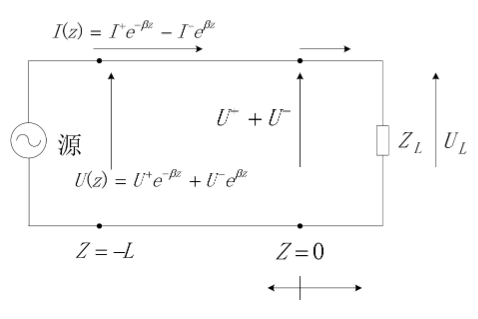
\includegraphics[width=0.4\linewidth]{pic/cb1_p1.png}
        \caption{}
    \end{center}
\end{figure}
\subsection{负载端($z=0$)处情况}
电压及电流为
\begin{align*}
     & U=U_L=U^++U^- \\
     & I=I_L=I^+-I^-
\end{align*}
而 $Z_0I^+=U^+,Z_0I^-=U^-$ ,公式可改写成
$$I_l=\dfrac{1}{Z_0}(U^+-U^-)$$
可得负载阻抗为
$$Z_L=\dfrac{U_L}{I_L}=Z_0\dfrac{U^++U^-}{I^+-I^-}$$
定义归一化负载阻抗为
$$z_L=\overline{Z_L}=\dfrac{Z_L}{Z_0}=\dfrac{1+\Gamma_L}{1-\Gamma_L}$$
其中定义 $\Gamma_L$ 为负载端的电压反射系数
$$\Gamma_L=\dfrac{U^-}{U^+}=\dfrac{\overline{Z_L}-1}{\overline{Z_L}+1}=|\Gamma_L|e^{\text{j}\varphi_L}$$
当 $Z_L=Z_0$ 或为无限长传输线时, $\Gamma_L=0$ ,无反射波,是行波状态或匹配状态。\\
当 $Z_L$ 为纯电抗元件或处于开路或者短路状态时, $|\Gamma_L|=1$ ,全反射,为驻波状态。\\
当 $Z_L$ 为其他值时, $|\Gamma_L|\leq 1$,为行波驻波状态。\\
线上任意点的反射系数为
$$\Gamma_L=|\Gamma_L|e^{\text{j}\varphi_L-\text{j}2\beta z}$$
定义驻波比 $VSWR$ 和回波损耗 $RL$ 为
\begin{align*}
     & VSWR=\dfrac{1+|\Gamma_L|}{1-|\Gamma_L|} \\
     & RL=-2\lg{|\Gamma_L|}
\end{align*}
\subsection{输入端($z=-L$)处情况}
反射系数 $\Gamma(z)$ 应改成
$$\Gamma(L)=\dfrac{U^-e^{-\text{j}\beta_L}}{U^+e^{\text{j}\beta_L}}=\dfrac{U^-}{U^+}e^{-\text{j}2\beta_L}=\Gamma_Le^{-\text{j}2\beta_L}$$
输入阻抗为
$$Z_{in}=Z_0\dfrac{Z_L+\text{j}Z_0\tan{\beta L}}{Z_0+\text{j}Z_L\tan{\beta L}}$$
由上式可知:
\begin{enumerate}
    \item 当 $L\to \infty$ 时, $Z_{in}\to Z_0$;
    \item 当 $\displaystyle L=\dfrac{\lambda}{2}$ 时, $Z_{in}=Z_L$;
    \item 当 $\displaystyle L=\dfrac{\lambda}{4}$ 时, $Z_{in}=\dfrac{Z_0^2}{Z_L}$.
\end{enumerate}
\section{实验设备}
\begin{enumerate}[label={\arabic*.}]
    \item 矢量网络分析仪\qquad 一台;
    \item 微带电路\qquad 一套。
\end{enumerate}
\section{实验内容}
\begin{enumerate}[label={\arabic*.}]
    \item 用矢量网络分析仪分别测量微带开路传输线模块的反射特性,并引入电阻负载、电容和电感负载测量,分析在不同负载情况下的反射特性;
    \item 用网络分析仪测量微带耦合滤波器的传输特性;
    \item 用网络分析仪测量天线的驻波比。
\end{enumerate}
\section{实验步骤及数据记录}
\subsection{开机}
打开网络分析仪电源,系统开机后需要先预热几分钟,等待仪器内器件稳定再开始测量。观察仪器面板和测量界面。
\subsection{选择测量内容}
按【测量】键,根据测试的内容选择显示面板右侧的按键,如按下[S11]软按键即测量反射,[S21]软按键即测量传输。
\subsection{选择测量格式}
按【格式】键,可选择测量结果显示的格式,如对数幅度,史密斯圆图等。
\subsection{设置频率范围}
矢量网络分析仪扫频工作,考虑到微带线设计的工作频率为2.5GHz,所以扫描频率可暂定为2.3GHz-2.7GHz,在测量过程中也可进一步调节频率范围。按【起始】键,然后用数字键和旁边的单位键输入测量的起始频率。此时测量界面下方显示的起始频率变为设置值。按【终止】键,然后用数字键和旁边的单位键输入测量的终止频率。此时测量界面下方显示的终止频率变为设置值。
\subsection{校准}
连接射频好电缆线之后,按【校准】键,出现多个校准选项,因为反射测量只需要用到矢网单个端口,为方便起见,可选择[机械校准]软按键,然后再选择[单端口(反射)]。此时显示面板右侧出现[开路器]、[短路器]和[负载],需要用配套的校准件,依次接上开路器、短路器和匹配负载,每接完一个校准件,就按下显示面板上相应选项右侧的软按键,显示选项下会出现下划线,如[开路器],则表示按键有效。最后按[完成单端口]软按键即完成校准,此时如果匹配负载校准件还未移除,可看到如图2显示测试界面,表示此时为史密斯圆图的匹配状态。
\begin{figure}[H]
    \begin{center}
        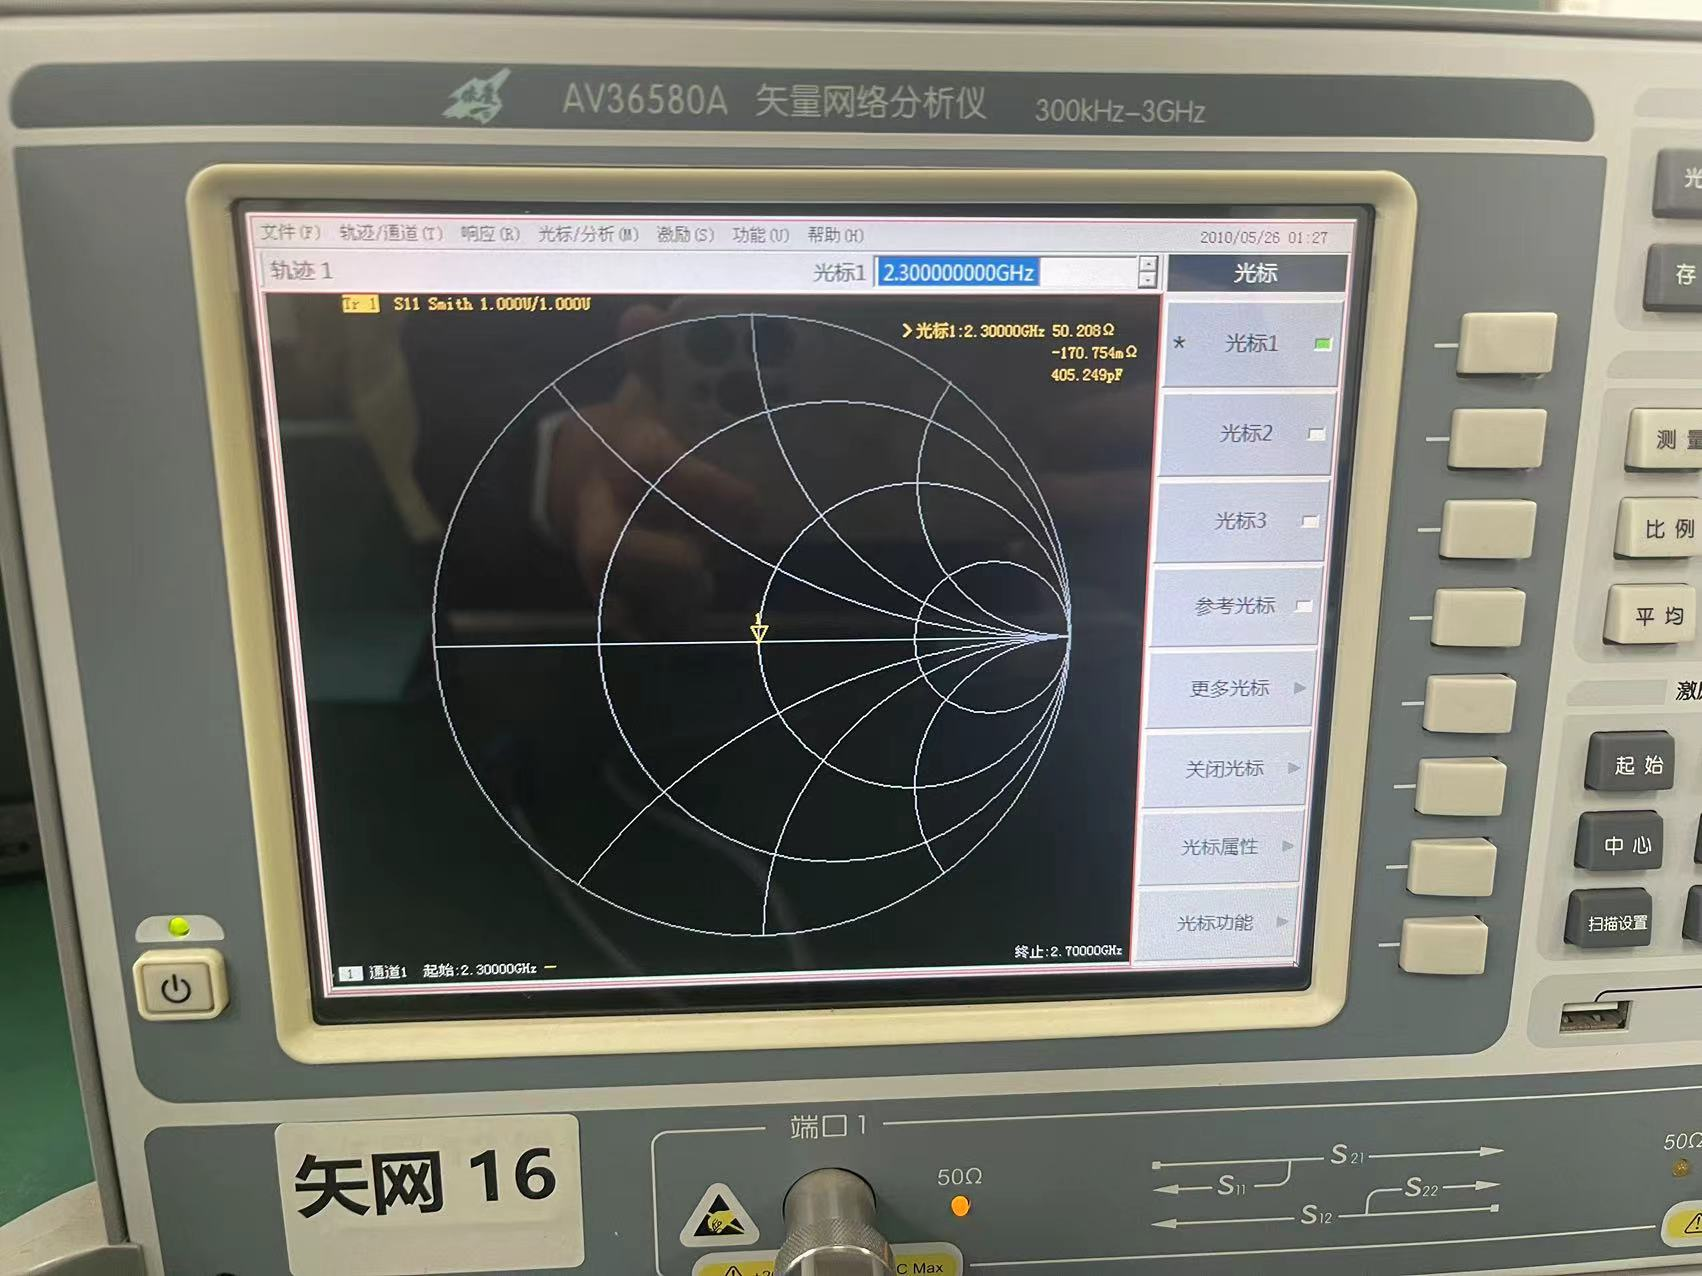
\includegraphics[width=0.4\linewidth]{pic/cb1_p2.jpg}
        \caption{}
    \end{center}
\end{figure}
\subsection{测量微带传输线电路模块}
在射频电缆线端接入微带开路传输线模块。然后按【光标】键打开光标,可看到类似图3的Smith曲线。旋转旋钮光标会沿着扫描曲线移动,同时可观察右上角的测量数据。
\begin{figure}[H]
    \begin{center}
        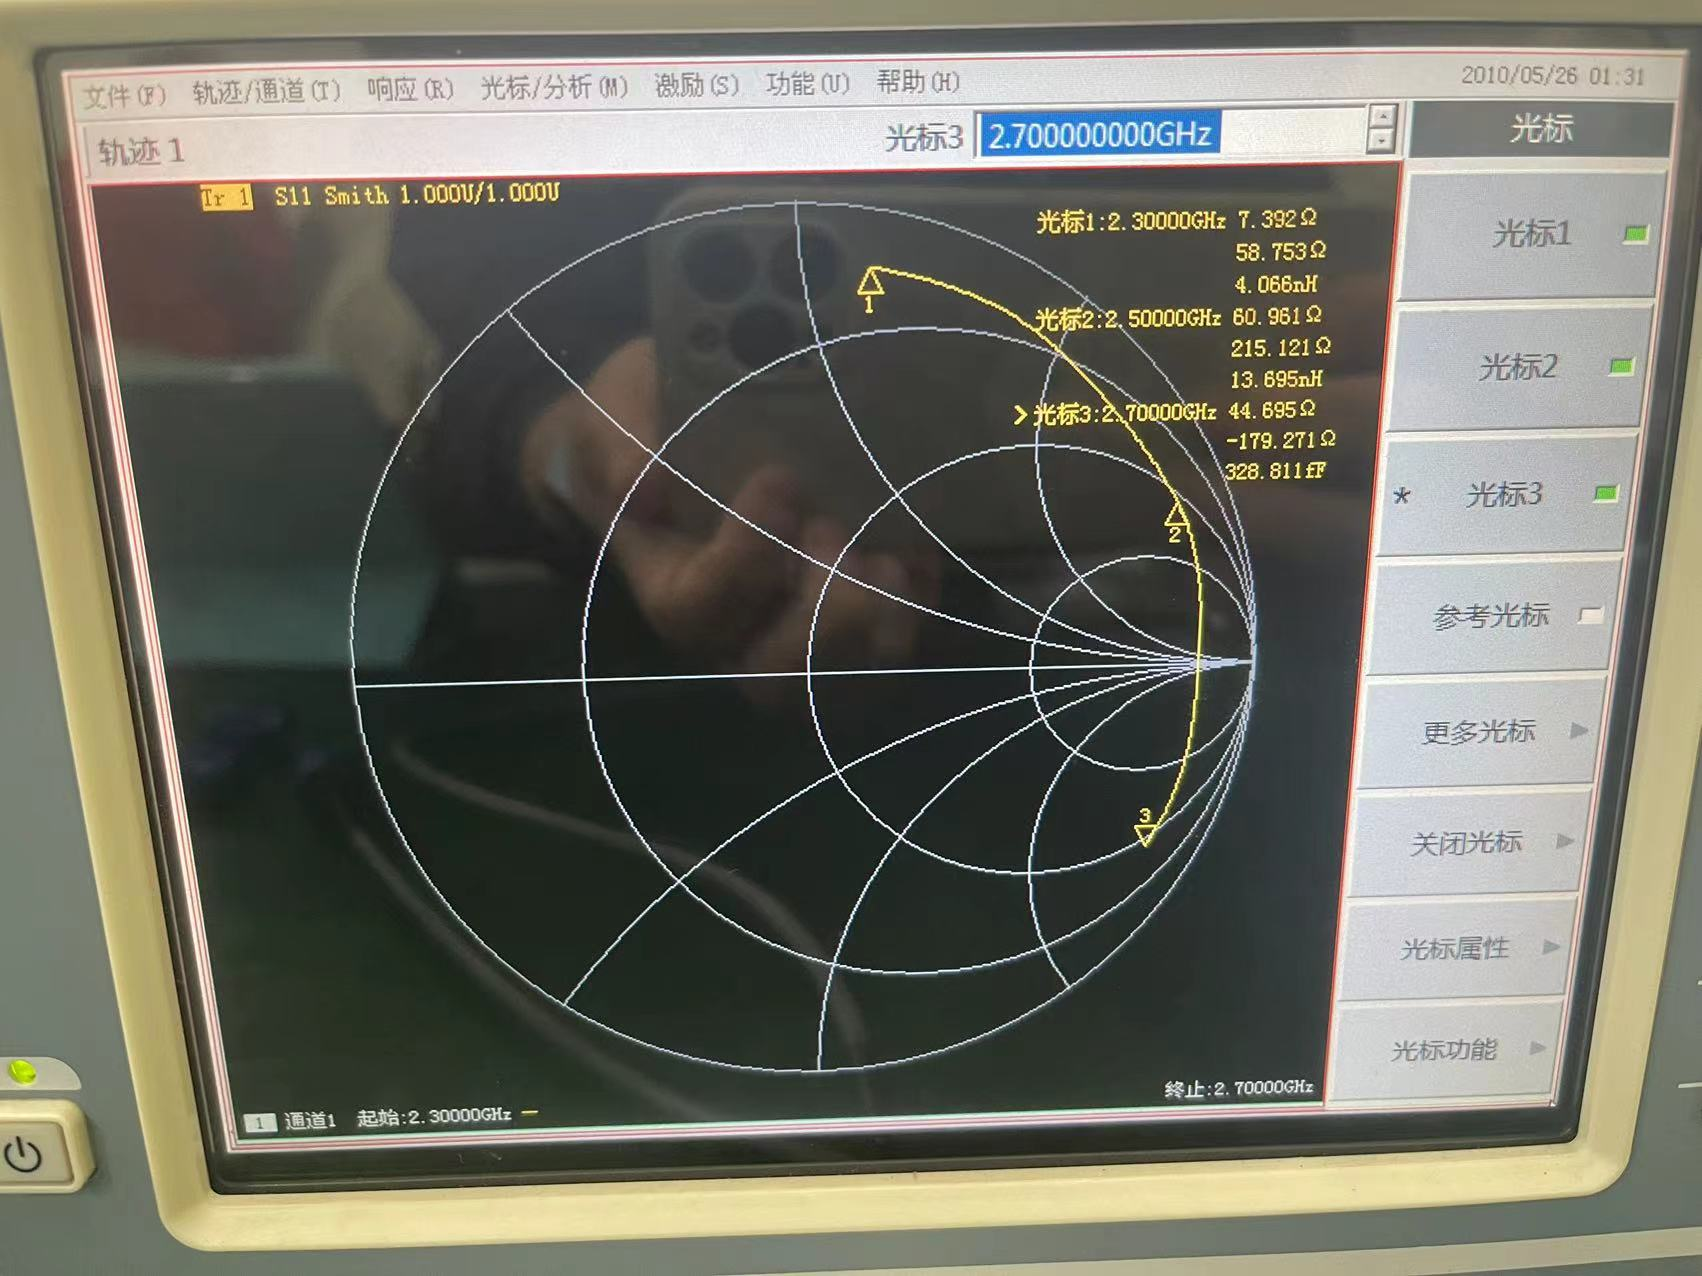
\includegraphics[width=0.4\linewidth]{pic/cb1_p3.jpg}
        \caption{}
    \end{center}
\end{figure}
\subsection{其他负载测量}
用防静电镊子夹取一个51欧姆阻值0805封装的贴片电阻,放置在测量模块的微带传输线末端,将电阻两端管脚分别架在传输线的开路端和覆铜接地端上,然后用镊子向下压紧使接触充分有效,观察此时网络分析仪测试窗口曲线的变化即为传输线负载端接入51欧姆电阻的情况。利用光标可观察各个频率上的反射情况如图4。
\begin{figure}[H]
    \begin{center}
        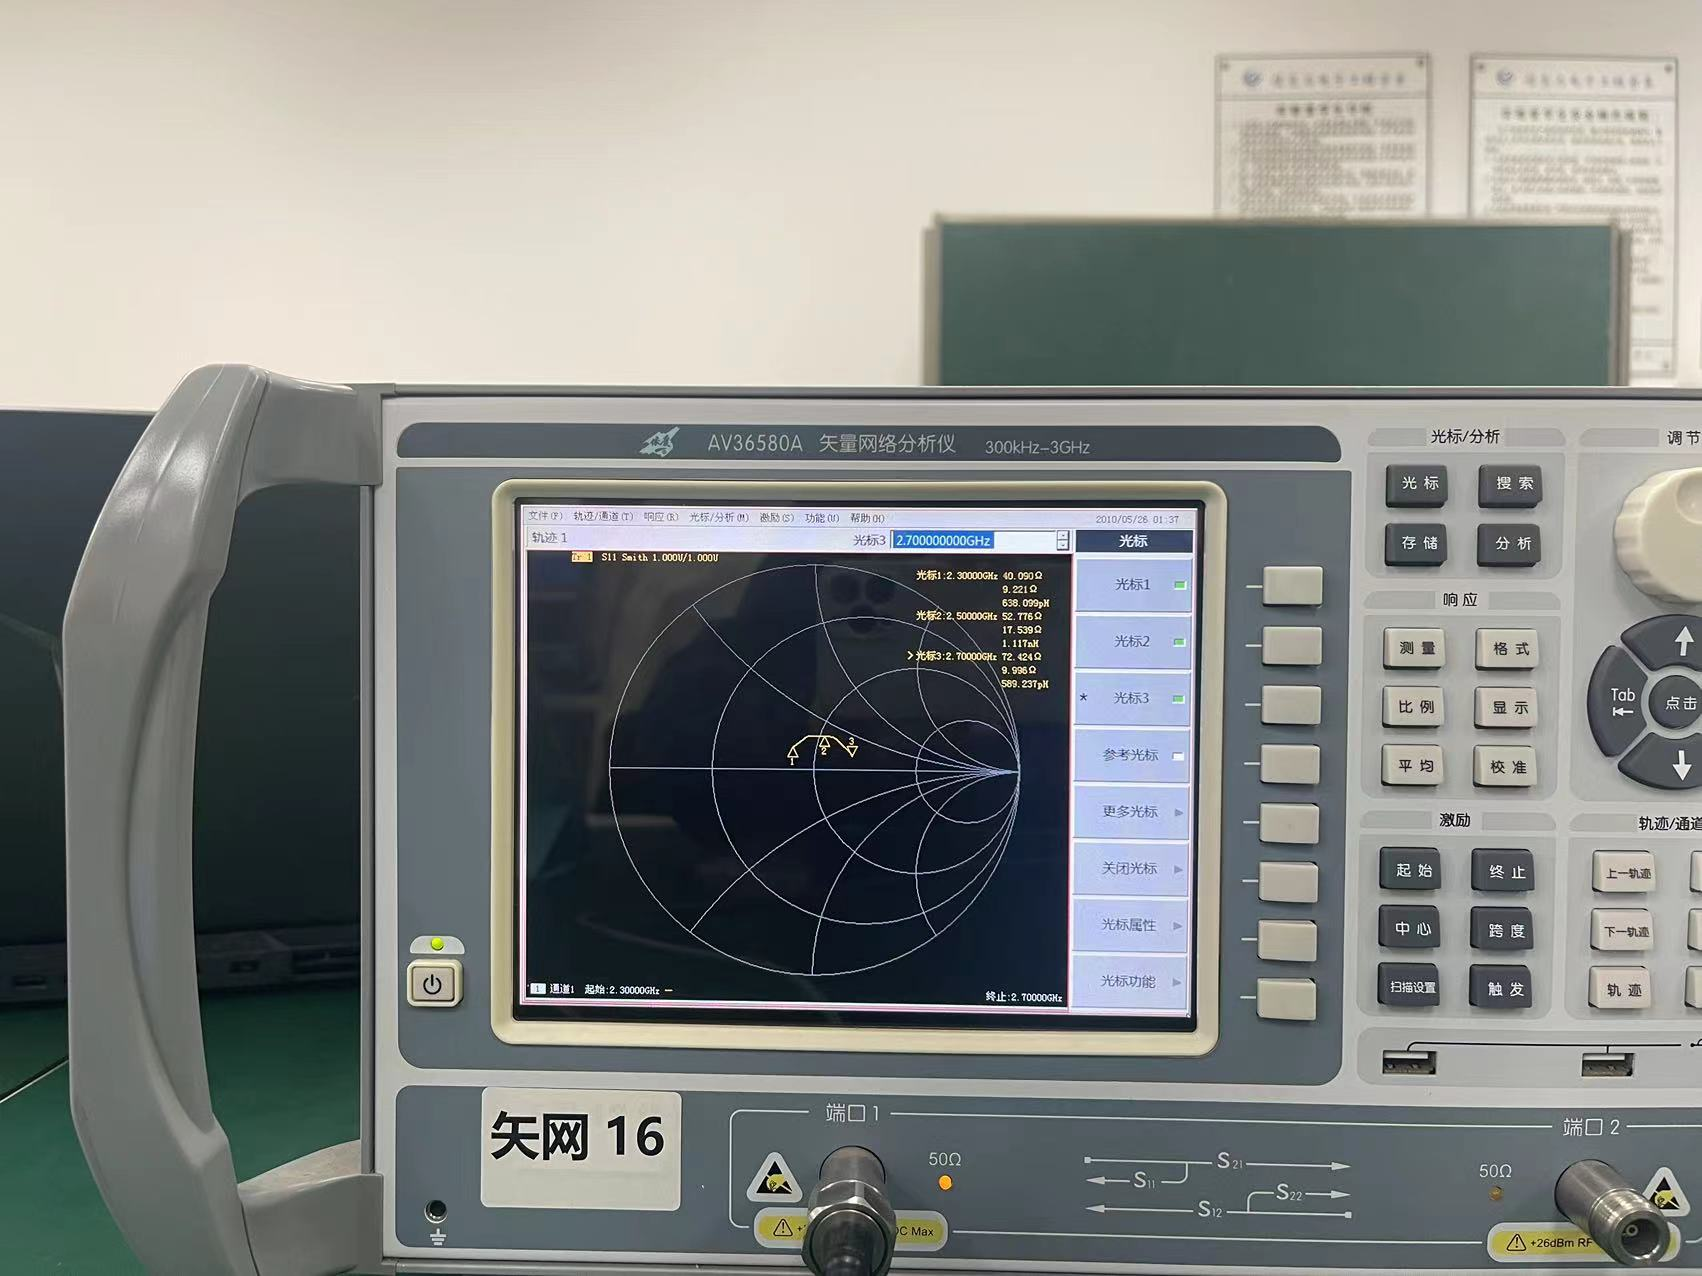
\includegraphics[width=0.4\linewidth]{pic/cb1_p4.jpg}
        \caption{}
    \end{center}
\end{figure}
同理测量短路、1pF电容、3.3nH电感的负载接入时的情况分别如图5、图6、图7所示:
\begin{figure}[H]
    \begin{center}
        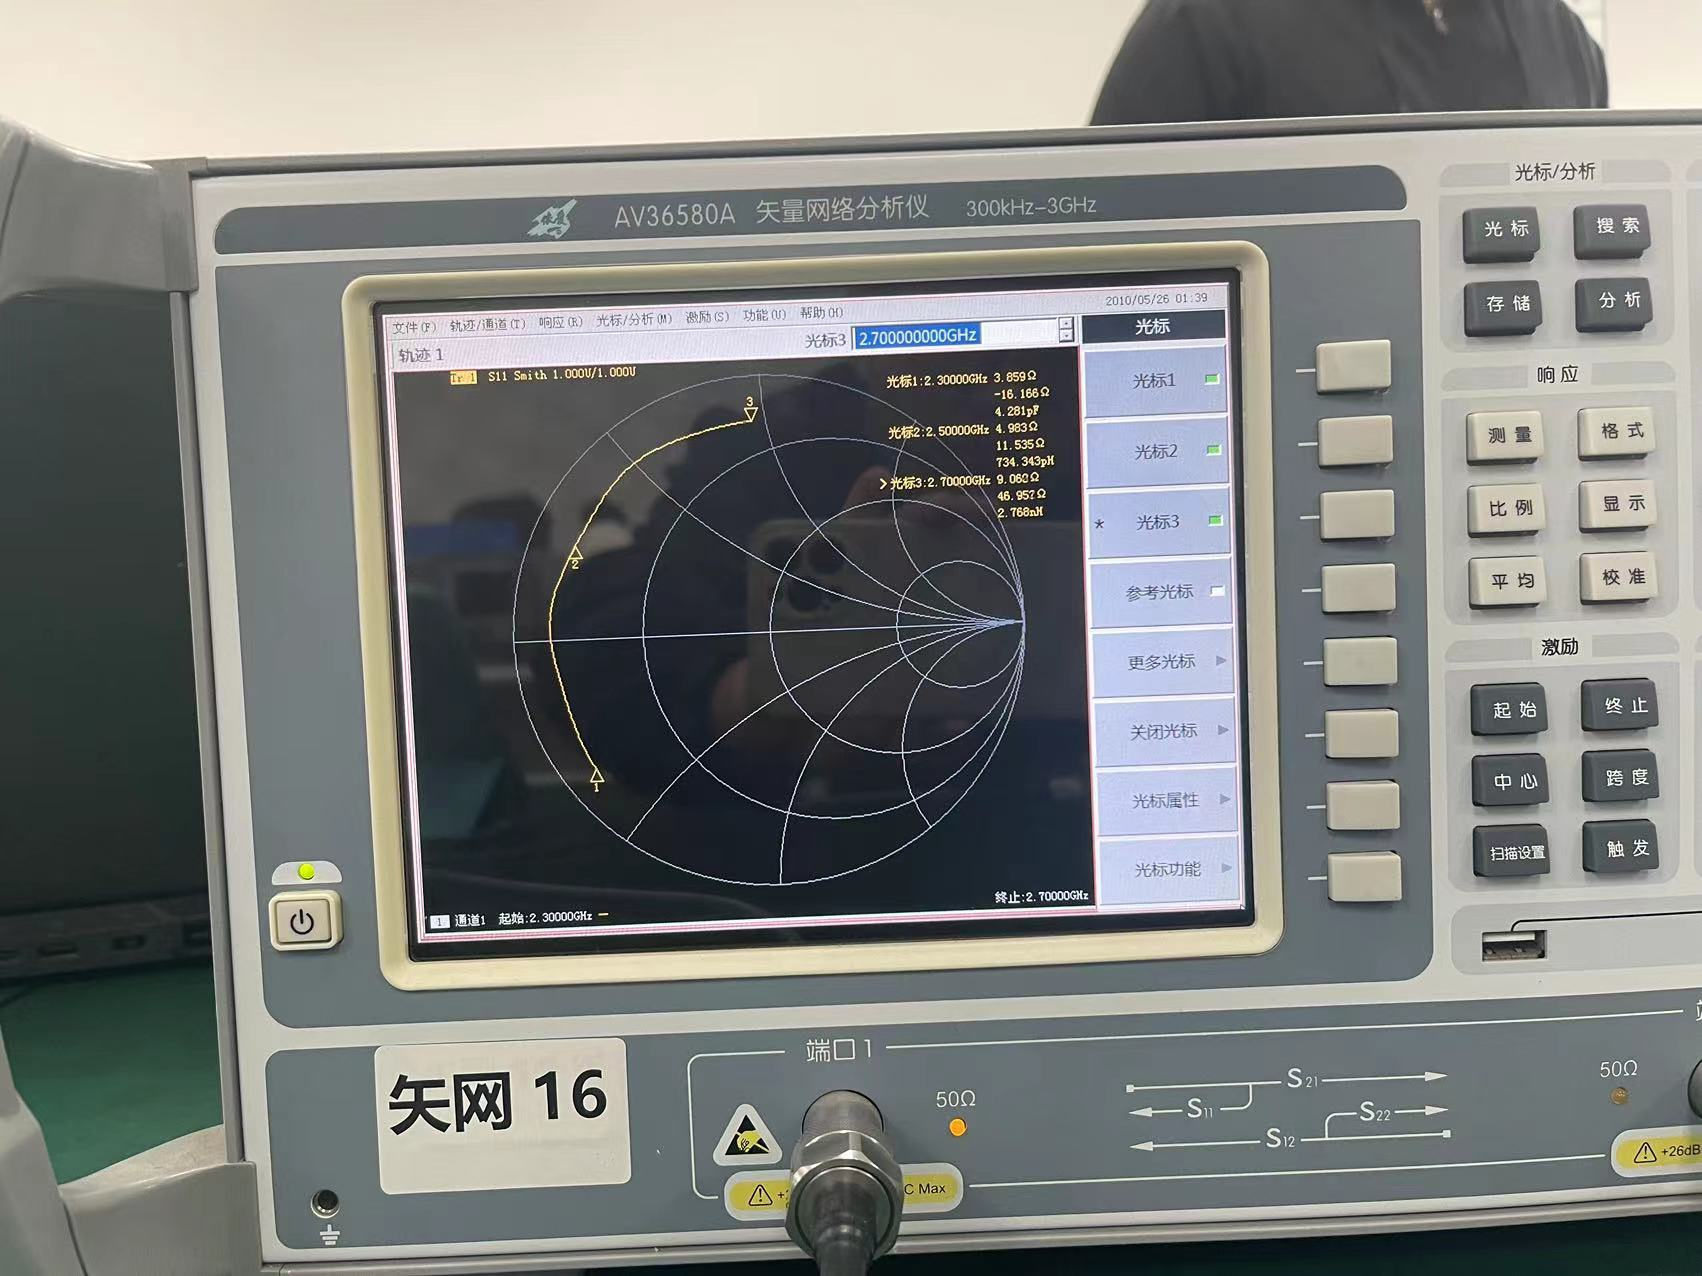
\includegraphics[width=0.4\linewidth]{pic/cb1_p5.jpg}
        \caption{}
    \end{center}
\end{figure}
\begin{figure}[H]
    \begin{center}
        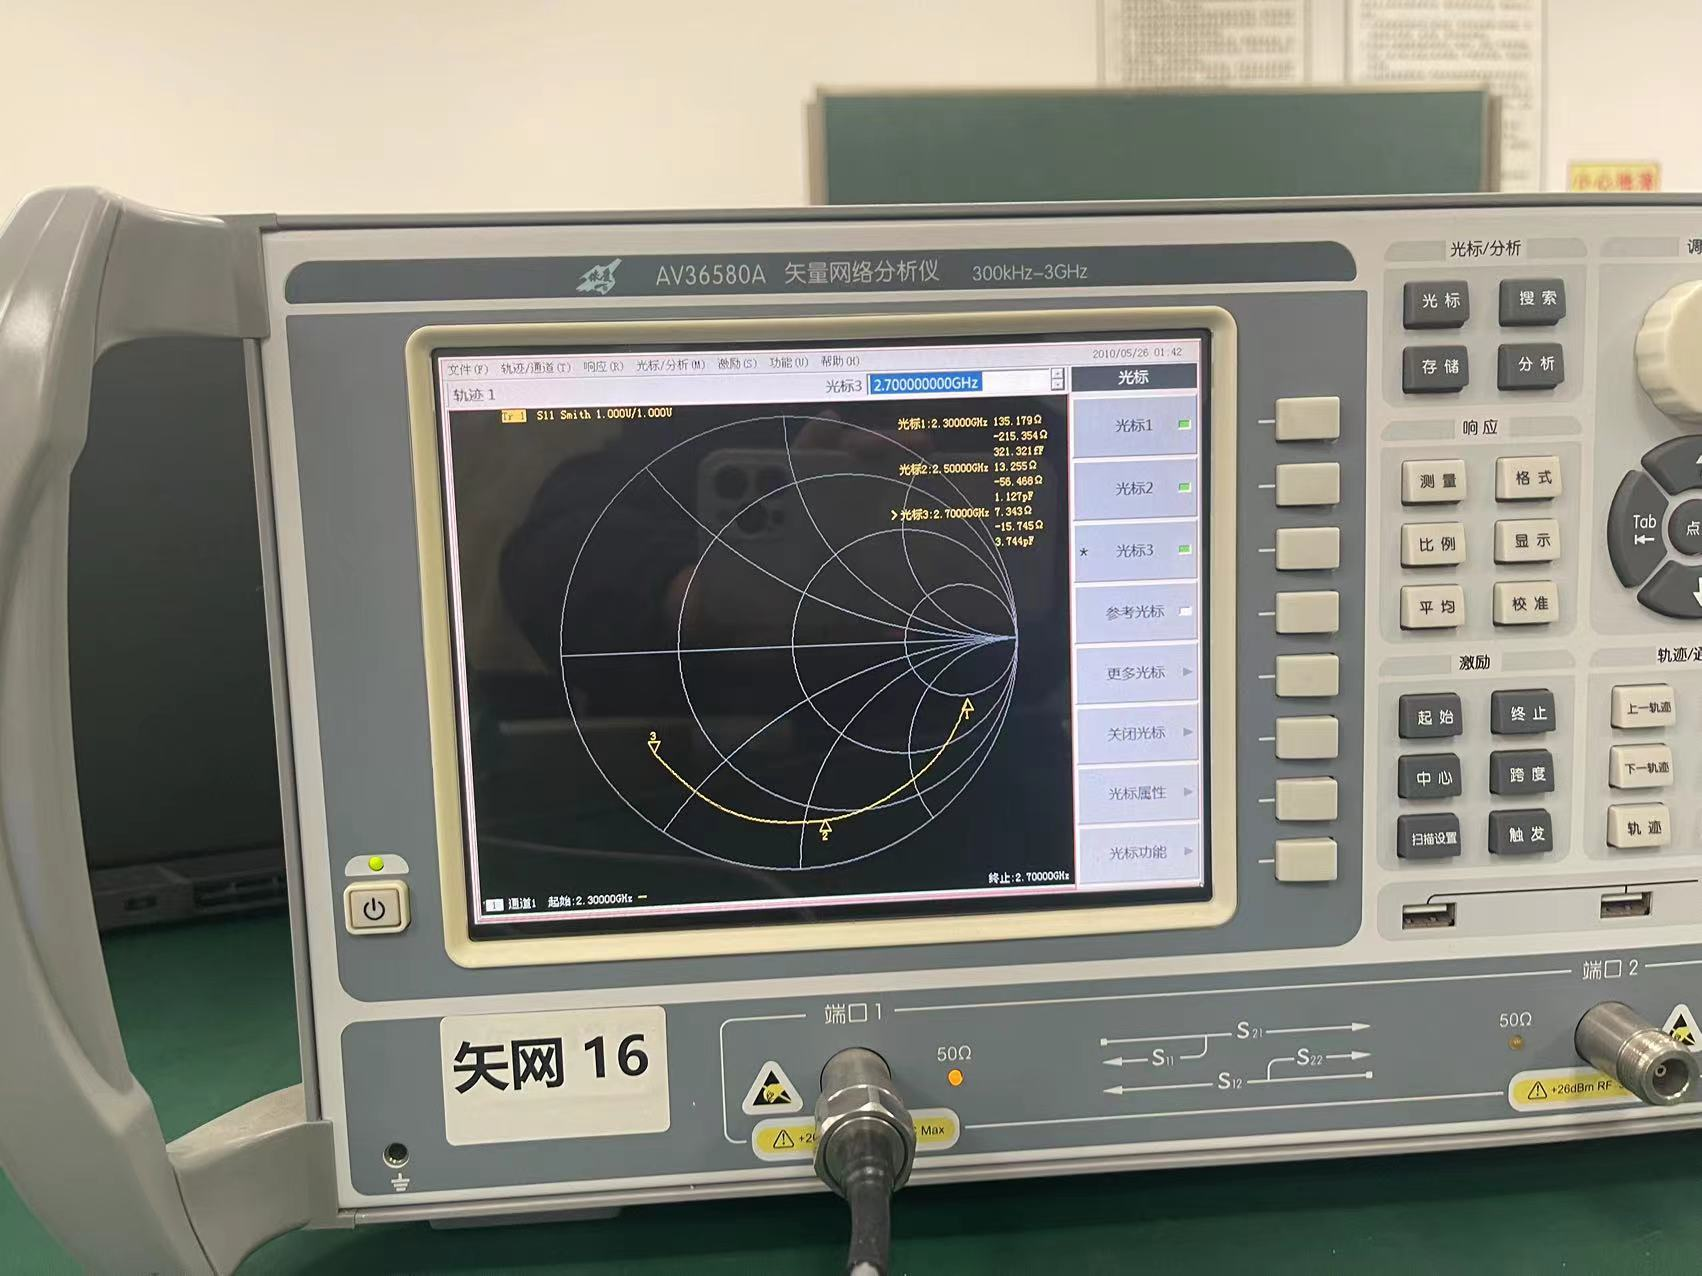
\includegraphics[width=0.4\linewidth]{pic/cb1_p6.jpg}
        \caption{}
    \end{center}
\end{figure}
\begin{figure}[H]
    \begin{center}
        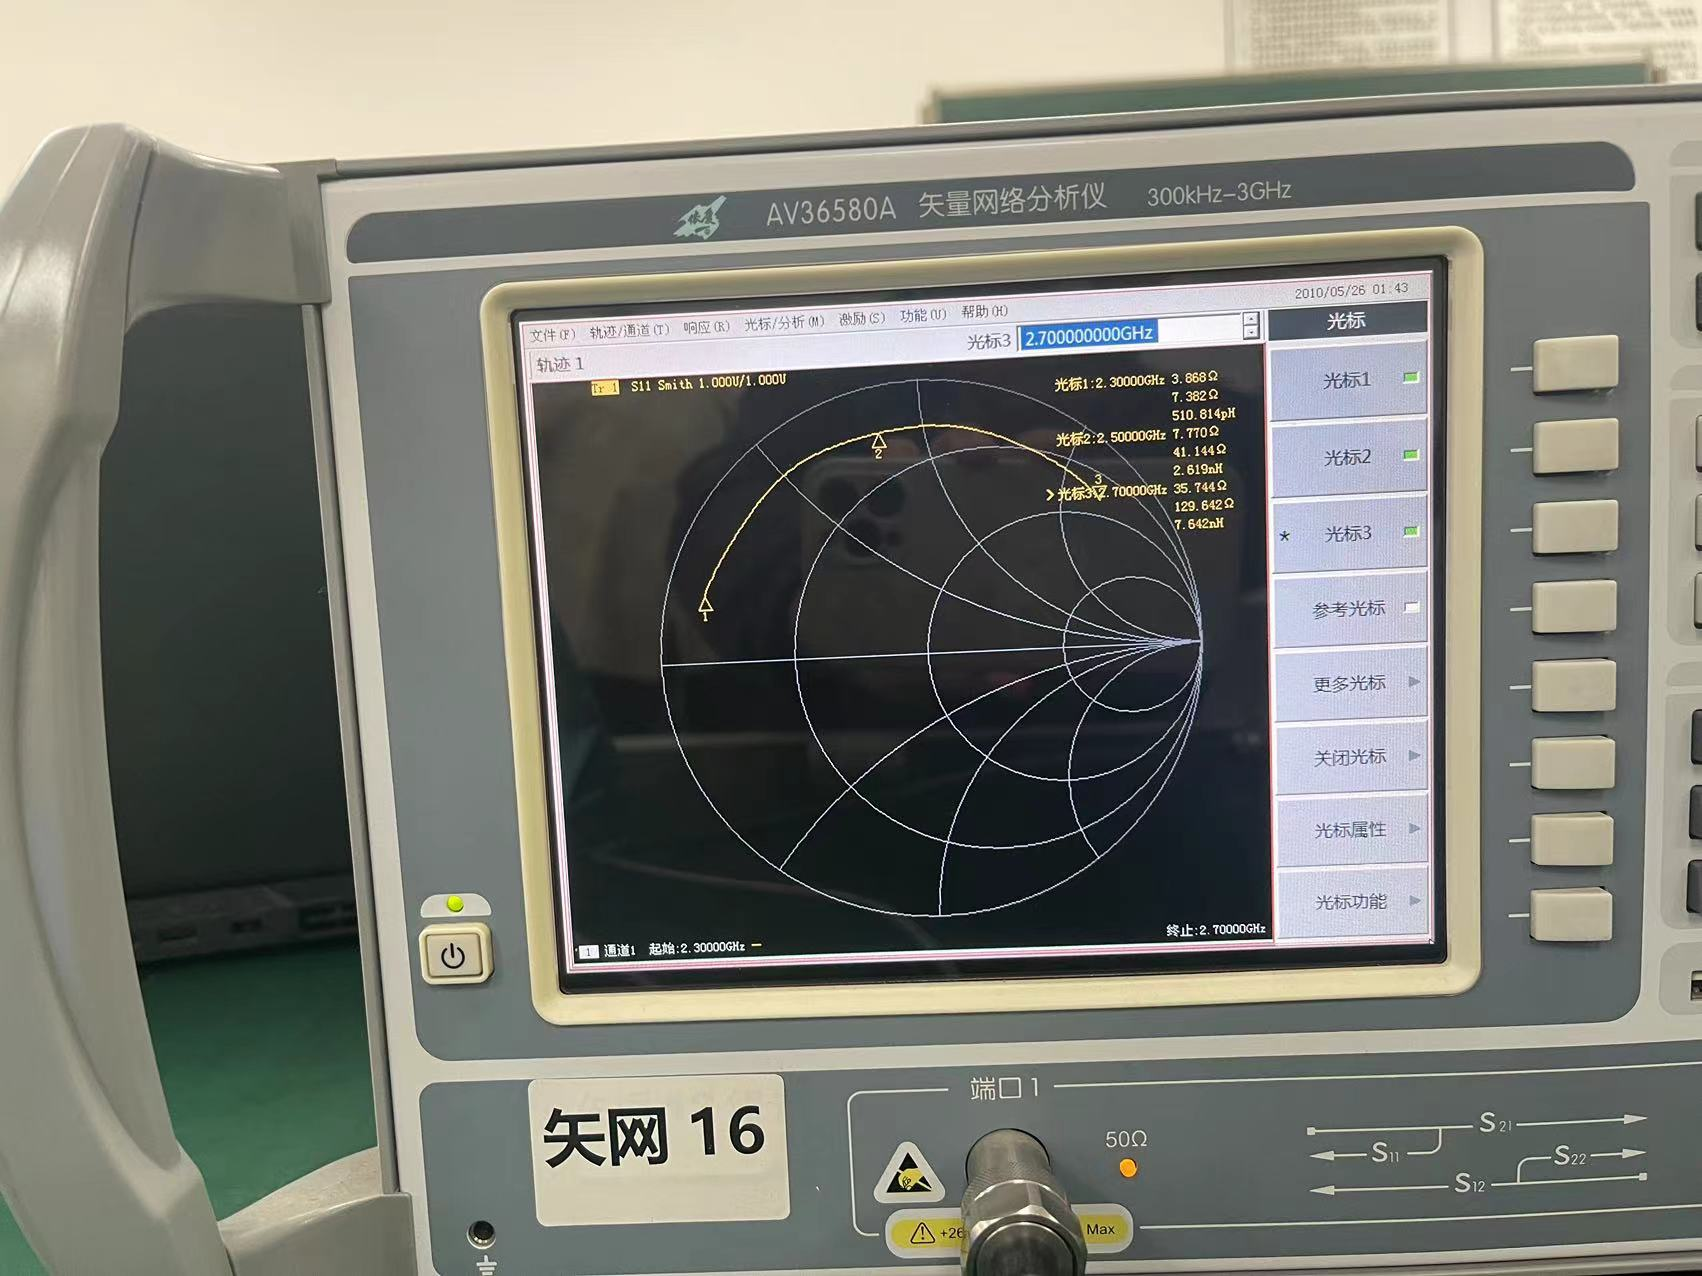
\includegraphics[width=0.4\linewidth]{pic/cb1_p7.jpg}
        \caption{}
    \end{center}
\end{figure}
\subsection{天线测量}
重新进行校准操作后将天线转接在网络分析仪端口处测量,测量结果的Smith圆图、对数幅度、驻波系数分别如图8、图9、图10:
\begin{figure}[H]
    \begin{center}
        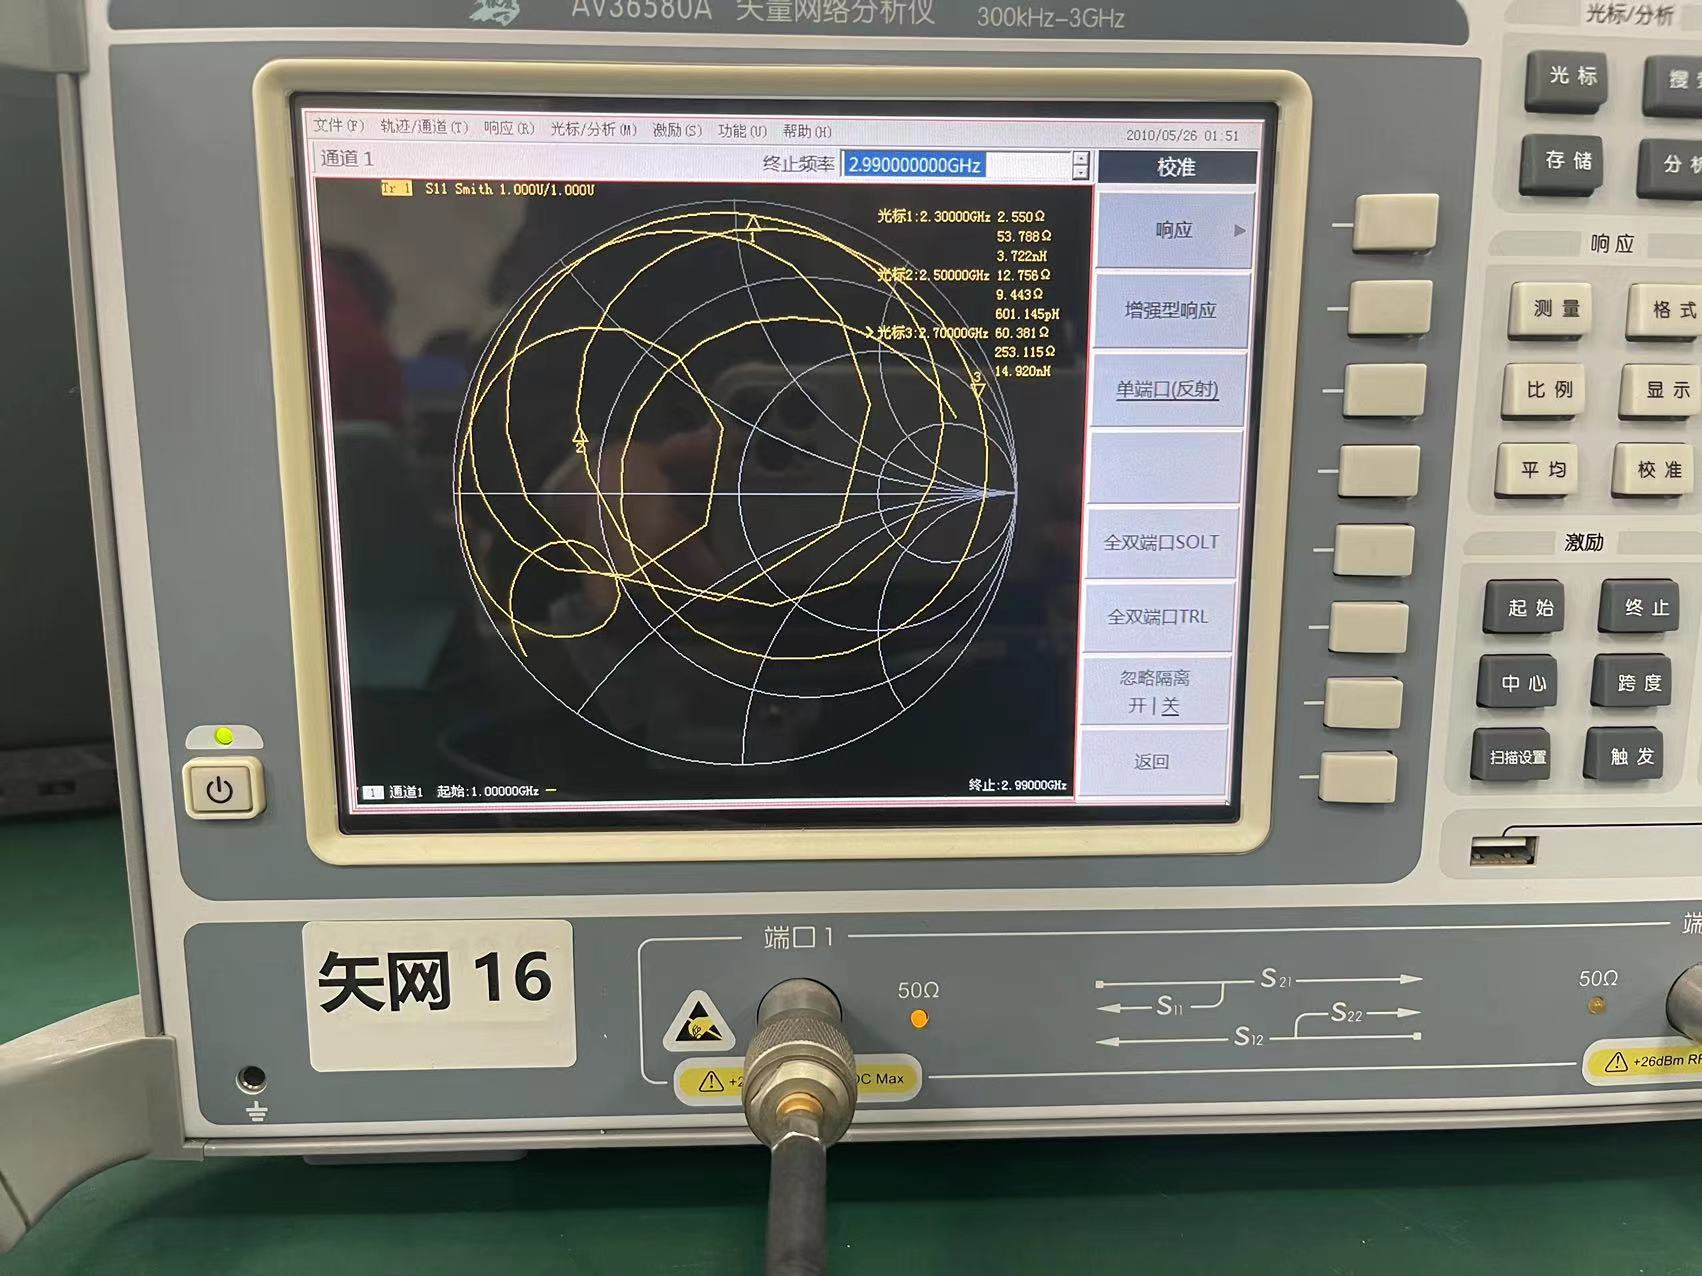
\includegraphics[width=0.35\linewidth]{pic/cb1_p8.jpg}
        \caption{}
    \end{center}
\end{figure}
\begin{figure}[H]
    \begin{center}
        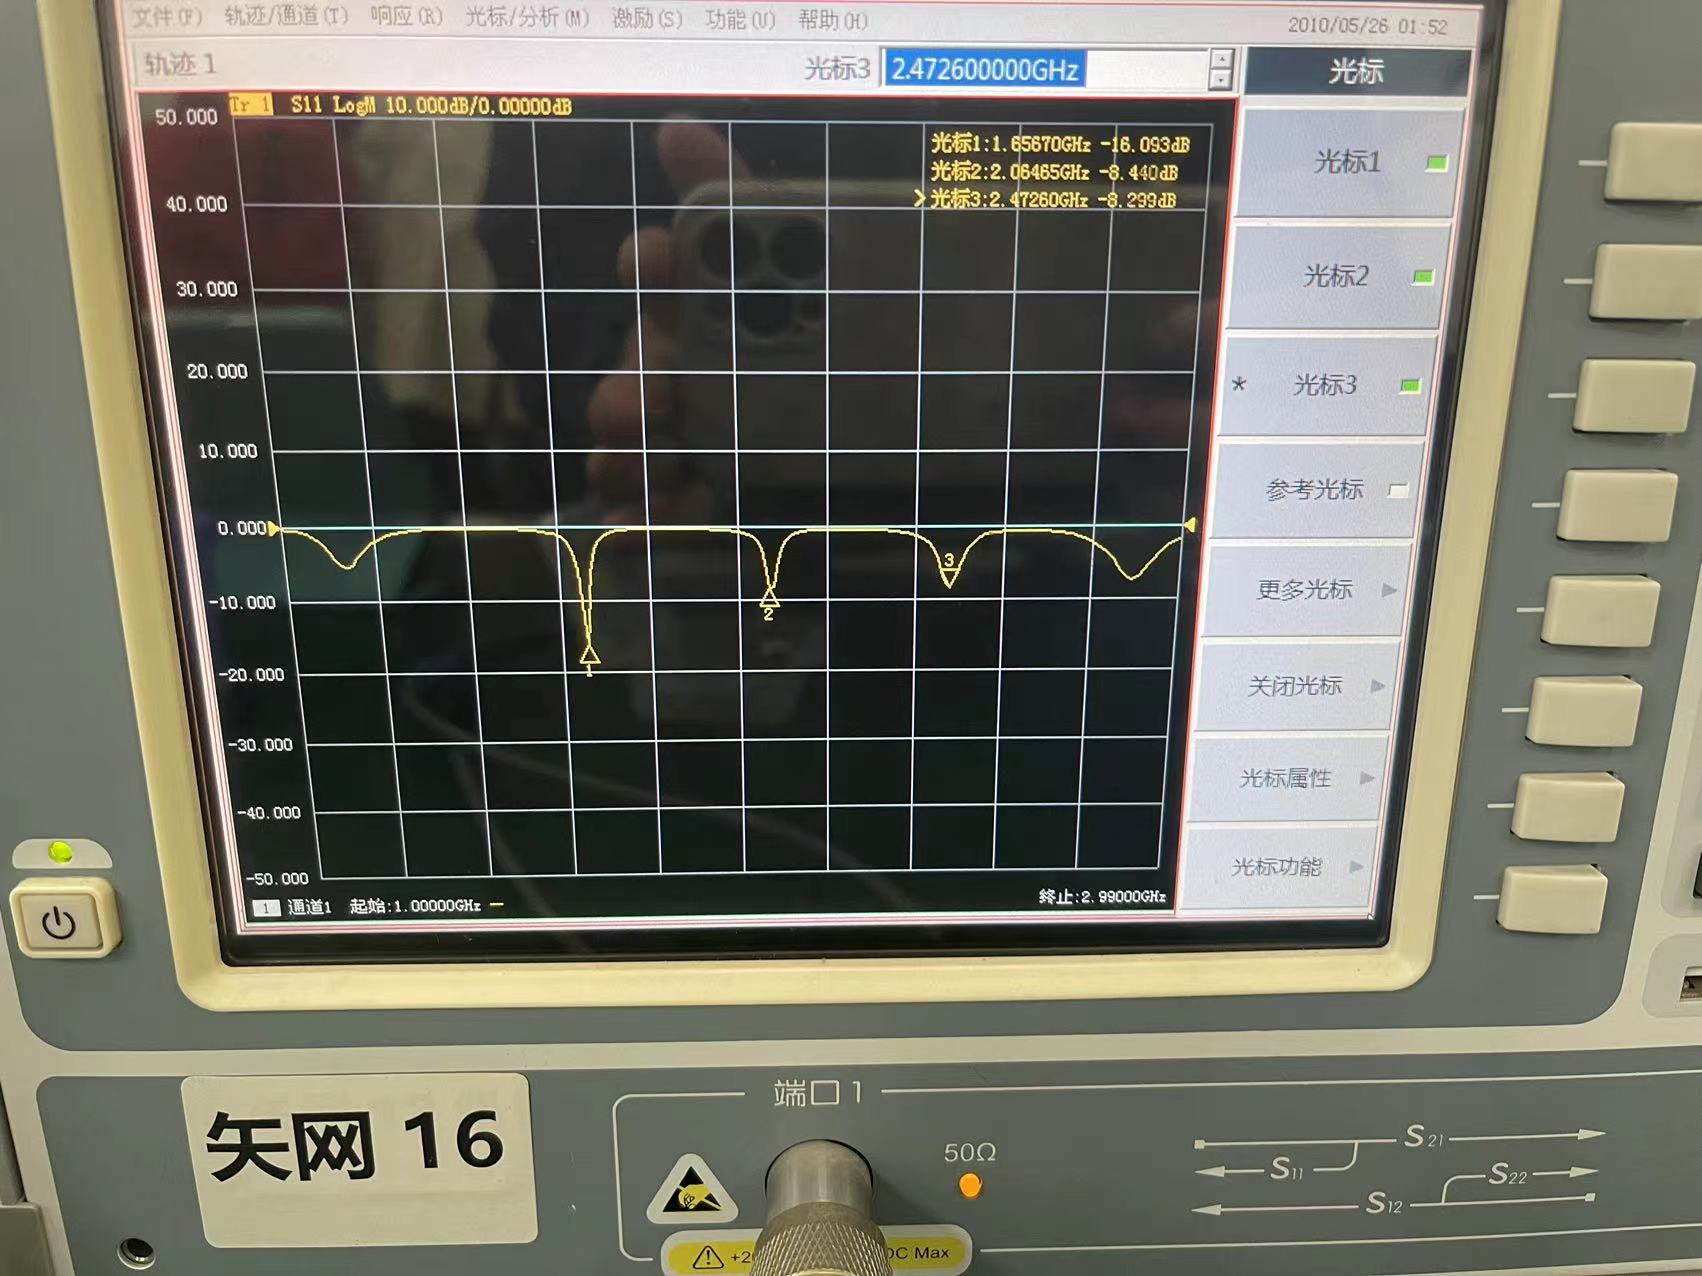
\includegraphics[width=0.35\linewidth]{pic/cb1_p9.jpg}
        \caption{}
    \end{center}
\end{figure}
\begin{figure}[H]
    \begin{center}
        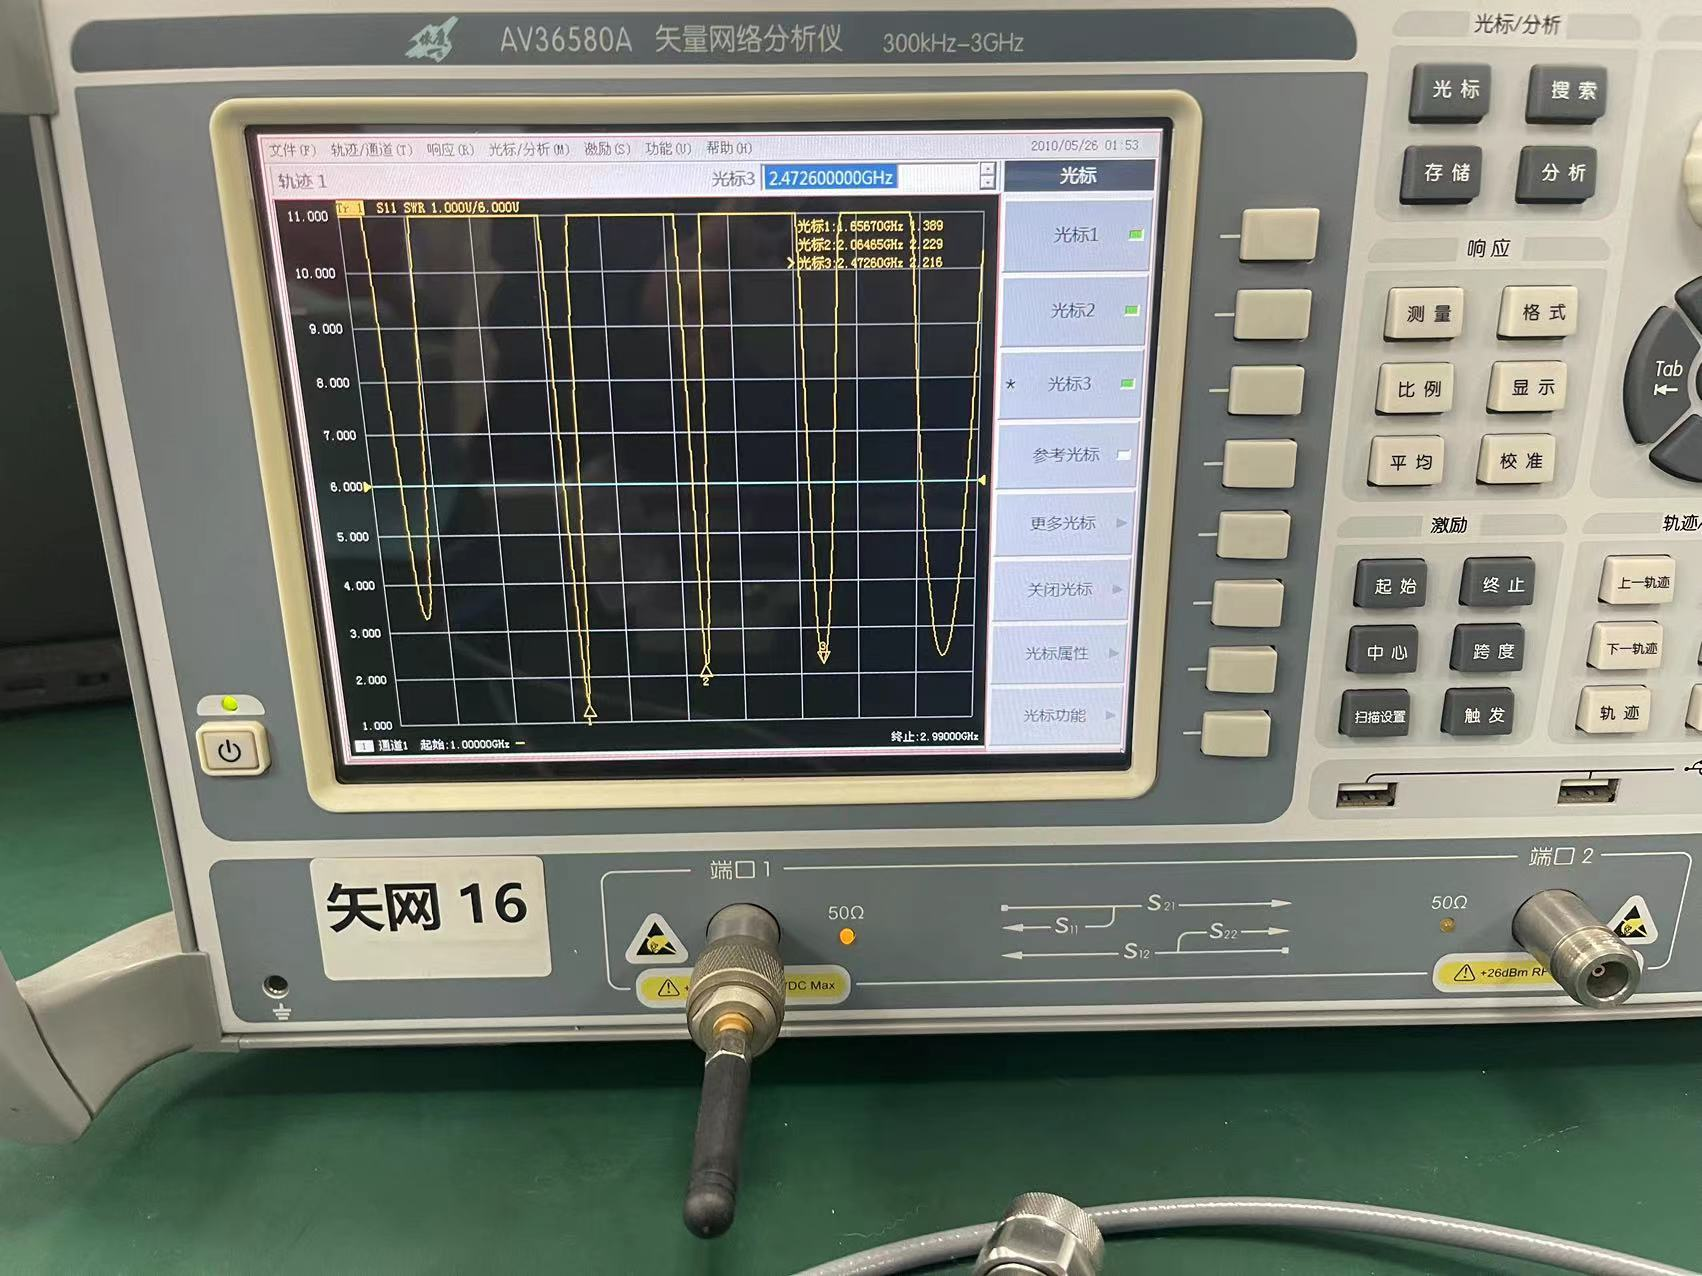
\includegraphics[width=0.4\linewidth]{pic/cb1_p10.jpg}
        \caption{}
    \end{center}
\end{figure}
\subsection{滤波器测量}
重新进行校准操作后将微带滤波器接在网络分析仪的两个端口测量S22,其幅度和相位特性分别如图11、图12:
\begin{figure}[H]
    \begin{center}
        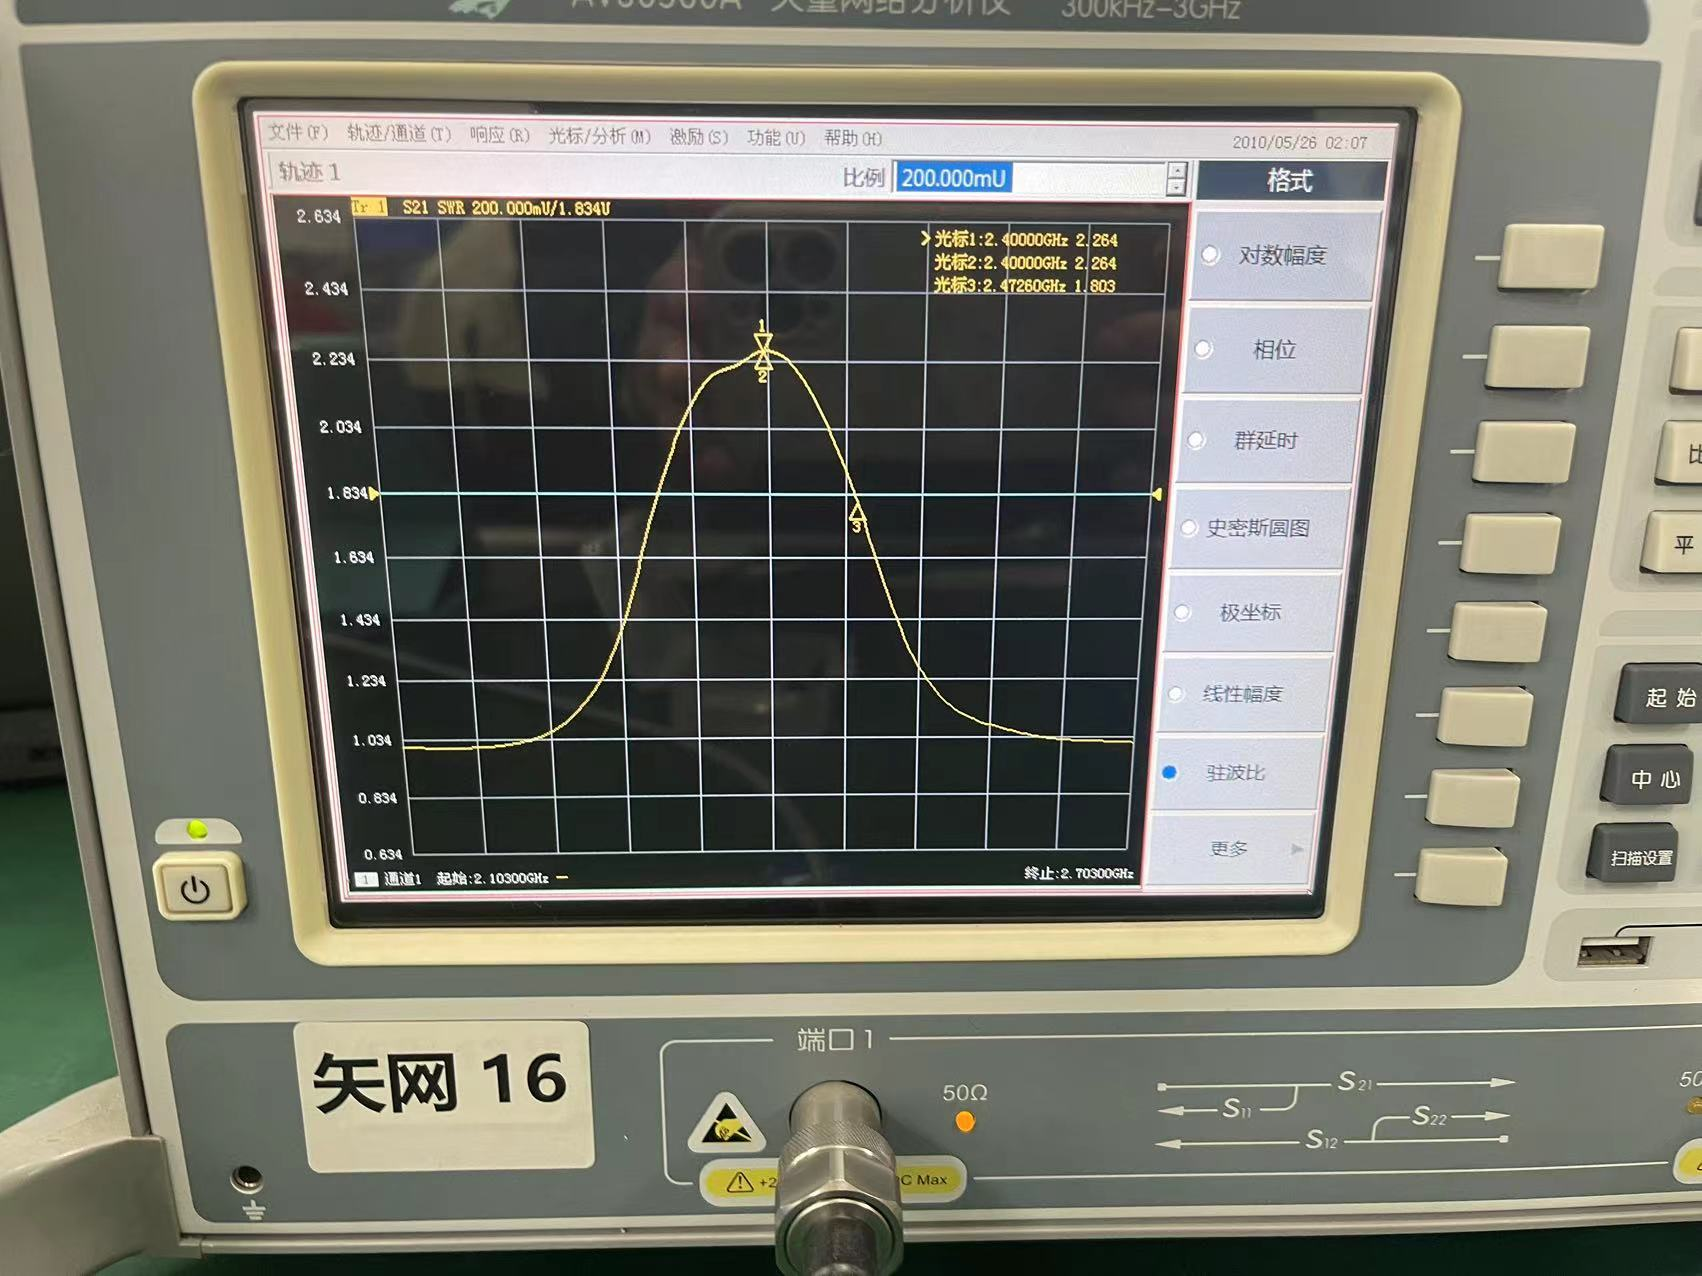
\includegraphics[width=0.35\linewidth]{pic/cb1_p11.jpg}
        \caption{}
    \end{center}
\end{figure}
\begin{figure}[H]
    \begin{center}
        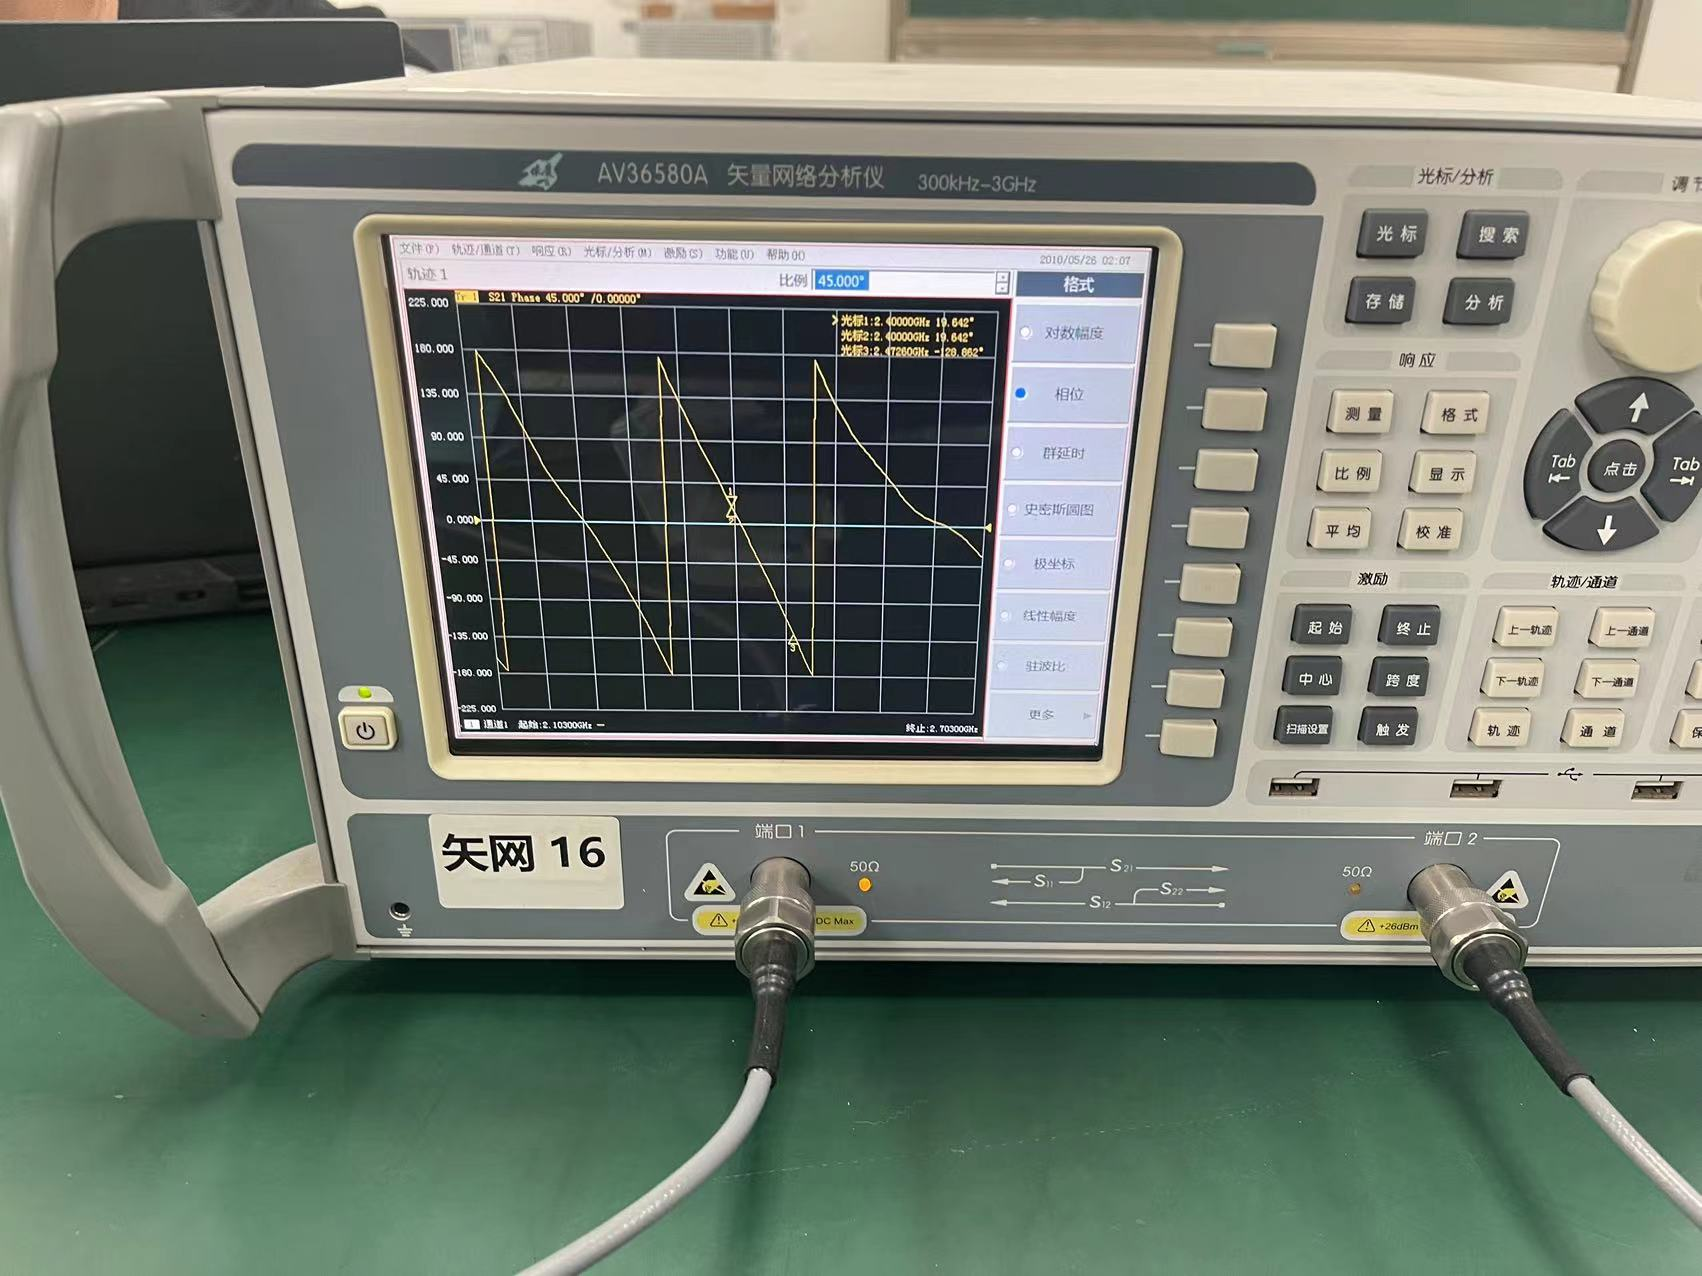
\includegraphics[width=0.35\linewidth]{pic/cb1_p12.jpg}
        \caption{}
    \end{center}
\end{figure}
\section{实验结果及分析}
\subsection{微带传输线测量}
根据实验原理,可计算理论值和测量实际值并进行如下对比:\par
\begin{table*}[h]
    \centering
    \begin{tabular}{|c|c|c|c|c|c|c|}
    \hline
    \multicolumn{2}{|c|}{\multirow{2}{*}{}} &\multirow{2}{*}{开路}&\multirow{2}{*}{短路} & \multirow{2}{*}{51Ω电阻}&\multirow{2}{*}{1pF电容} & \multirow{2}{*}{3.3nH电感}\\
    \multicolumn{2}{|c|}{\multirow{2}{*}{}} & & & & & \\
    \hline
    \multirow{3}{*}{理论值} & 2.3GHz & $1\angle 0^{\circ}$ & $1\angle 180^{\circ}$ & $0.0099\angle 0^{\circ}$ & $1\angle -13.120^{\circ}$ & $0.999\angle 162.737^{\circ}$ \\
    \cline{2-7}
    \multirow{3}{*}{}  & 2.5GHz & $1\angle 0^{\circ}$ & $1\angle 180^{\circ}$ & $0.0099\angle 0^{\circ}$ & $1\angle -14.250^{\circ}$ & $0.999\angle 161.261^{\circ}$ \\
    \cline{2-7}
    \multirow{3}{*}{} & 2.7GHz & $1\angle 0^{\circ}$ & $1\angle 180^{\circ}$ & $0.0099\angle 0^{\circ}$ & $0.999\angle -15.377^{\circ}$ & $1\angle 159.792^{\circ}$ \\
    \hline
    \multirow{3}{*}{实际值} & 2.3GHz & $0.884\angle 80.278^{\circ}$ & $0.869\angle -143.984^{\circ}$ & $0.148\angle 119.732^{\circ}$ & $0.825\angle -19.328^{\circ}$ & $0.859\angle 163.106^{\circ}$ \\
    \cline{2-7}
    \multirow{3}{*}{}  & 2.5GHz & $0.890\angle 24.368^{\circ}$ & $0.827\angle 153.779^{\circ}$ & $0.177\angle 58.255^{\circ}$ & $0.805\angle -81.585^{\circ}$ & $0.831\angle 100.288^{\circ}$ \\
    \cline{2-7}
    \multirow{3}{*}{} & 2.7GHz & $0.885\angle -29.539^{\circ}$ & $0.826\angle 92.596^{\circ}$ & $0.202\angle 8.017^{\circ}$ & $0.776\angle -144.744^{\circ}$ & $0.839\angle 39.756^{\circ}$ \\
    \hline
    \end{tabular}
\end{table*}
可以发现理论值与实际值之间的 $|\Gamma|$ 均相差0.2左右,推测是由于微带传输线模块本身与矢量网络分析仪之间连接部分不止 $\displaystyle \dfrac{\lambda}{2}$ ,导致实际的 $|\Gamma|$ 测得值之间有偏差。
\subsection{天线测量}
测量结果的幅度、驻波系数特性见上方的图9、图10.
\subsection{滤波器测量}
从图11、图12的幅度和相位特性中可以看出其中心频率 $f_0=\text{2.4GHz}$ ,3dB带宽 $\Delta = 0.24GHz$ ,回波损耗 $\displaystyle RL={20\lg\dfrac{VSMR+1}{VSMR-1}}=8.24\text{dB}$ ,阻带衰减6.81dB.由此可见该滤波器通频带较宽,回波损耗较大,因此性能较好。
\section{思考题}
\subsection{什么是 $S$ 参数?}
$S$ 参数,也就是散射参数。是微波传输中的一个重要参数。 $S_{12}$ 为反向传输系数,也就是隔离。 $S_{21}$ 为正向传输系数,也就是增益。 $S_{11}$为输入反射系数,也就是输入回波损耗, $S_{22}$ 为输出反射系数,也就是输出回波损耗。
\subsection{如果不校准,直接接入射频电缆和电路模块测量会对结果有什么影响?}
电缆的阻抗会对最终结果造成影响,使得到的史密斯圆图会不光滑,边缘参差不齐,即测出的数据不准确。
\subsection{如何测量转接头对测试曲线的影响?}
可以用完全匹配的负载阻抗进行测试,校准后矢量网络分析仪距离圆心的误差就是转接头产生的误差。
\subsection{利用实验内容2中已知的设计参数,计算50欧半波长微带线的长度和宽度。}
由工作频率 $f=2.5\text{GHz}$ 可知其波长
$$\lambda=\dfrac{c}{f}=0.12\text{m}$$
因此半波长微带线的长度为
$$L=\dfrac{\lambda}{2}=0.06\text{m}$$
已知微带线长度计算公式
$$ L=(5.8H+1.7W+1.25G+0.25\pi D)(1-0.64\varepsilon) $$
其中, $L$ 为微带线的长度, $H$ 为微带线的高度, $W$ 为微带线的宽度, $G$ 为微带线与接地铺铜的间隙, $D$ 为微带线的直径, $\varepsilon$ 为介电常数。公式中的单位为毫米。\\
带入计算可得微带线宽度
$$ W=32.658\text{mm} $$
\section{讨论与心得}
\subsection{实验收获与体会}
在本次实验中,我对前些天课程学的传输线方程、Smith圆图的理论知识进行了复习,并学习了如何使用矢量网络分析仪,将理论与实践相结合,在加深对理论知识理解的同时为以后做射频与微波方面的研究打下了实践的基础。但是,在本次实验中由于个人的疏忽导致测量的数据量较少,下次应该改正该错误,在实验前仔细阅读实验要求。
\subsection{实验建议与意见}
希望下次实验要求能够更加明确详细一点,并且对如何在矢量网络分析仪上读取数据的说明更加详细一点。
\end{document}